\documentclass[12pt]{article}
\usepackage{amsmath}
\usepackage{listings}
\usepackage{color}
\usepackage{graphicx}
\usepackage[margin=0.5in]{geometry}

\title{Homework 1}
\author{Dan Kolbman}
\date{September 19, 2014}

\definecolor{mygreen}{rgb}{0,0.6,0}
\definecolor{mygray}{rgb}{0.95,0.95,0.95}
\definecolor{mymauve}{rgb}{0.58,0,0.82}
%\definecolor{mygray}{RGB}{22, 22, 22}}

\lstset{ %
  language=Python,
  backgroundcolor=\color{mygray},   % choose the background color
  basicstyle=\footnotesize,        % size of fonts used for the code
  breaklines=true,                 % automatic line breaking only at whitespace
  captionpos=b,                    % sets the caption-position to bottom
  commentstyle=\color{mygreen},    % comment style
  %escapeinside={\%*}{*)},          % if you want to add LaTeX within your code
  keywordstyle=\color{blue},       % keyword style
  stringstyle=\color{mymauve},     % string literal style
  frame=L,
  xleftmargin=\parindent,
  showstringspaces=false
}
\begin{document}
  
  \maketitle
 
  \section{Break math:}
  Rounding errors in Python's sqrt() function:
  \lstinputlisting[language=Python]{Problem1.py}
  Output:
  \lstinputlisting{Problem1.out}
  
  \clearpage

  \section{Matrix inversion via libraries and research:}
  Using numpy:
  \lstinputlisting[language=Python]{Problem2.py}
  Output:
  \lstinputlisting{Problem2.out}
  
  \section{Binary and Floating point notation:}
  $10.5 =         0|10000000010|1.0101\overline{0}_2$\\\\
  $\frac{1}{3} =  0|01111111101|1.\overline{01}_2$\\\\
  $\frac{22}{7} = 0|10000000000|1.\overline{1001}_2$
  
  \clearpage

  \section{Head-to-Head}
  Find zero of $f(x) = x^4 - 2$ using Bisection, Secant, False Position,
  and Fixed Point Iteration.

  \subsection{Bisection}
  \lstinputlisting[language=Python, firstline=2,lastline=29]{Problem4a.py}
  \begin{figure}[h!]
    \centering
    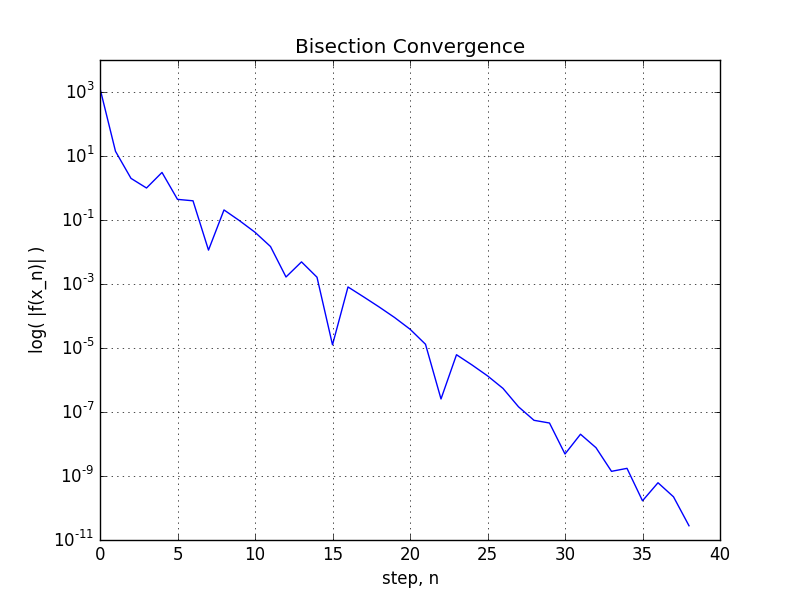
\includegraphics[width=0.5\textwidth]{Problem4a.png}
    \caption{(Approximately) Quadratic Convergence}
  \end{figure}

  \clearpage
  
  \subsection{Secant Method}
  \lstinputlisting[language=Python, firstline=2, lastline=22]{Problem4b.py}
  \begin{figure}[h!]
    \centering
    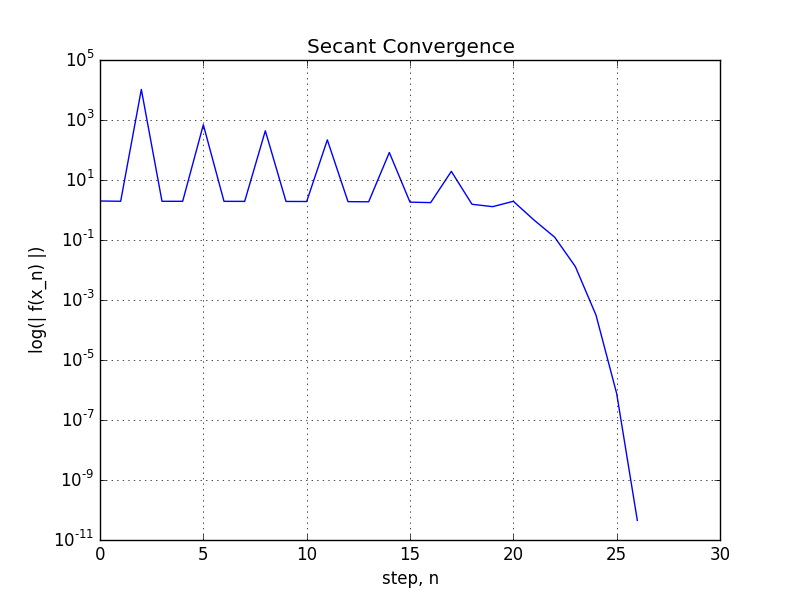
\includegraphics[width=0.8\textwidth]{Problem4b.png}
    \caption{Takes a couple of iterations before the root is properly bracketted}
  \end{figure}


  \clearpage

  \subsection{False Position Method}
  \lstinputlisting[language=Python, firstline=2, lastline=28]{Problem4c.py}
  \begin{figure}[h!]
    \centering
    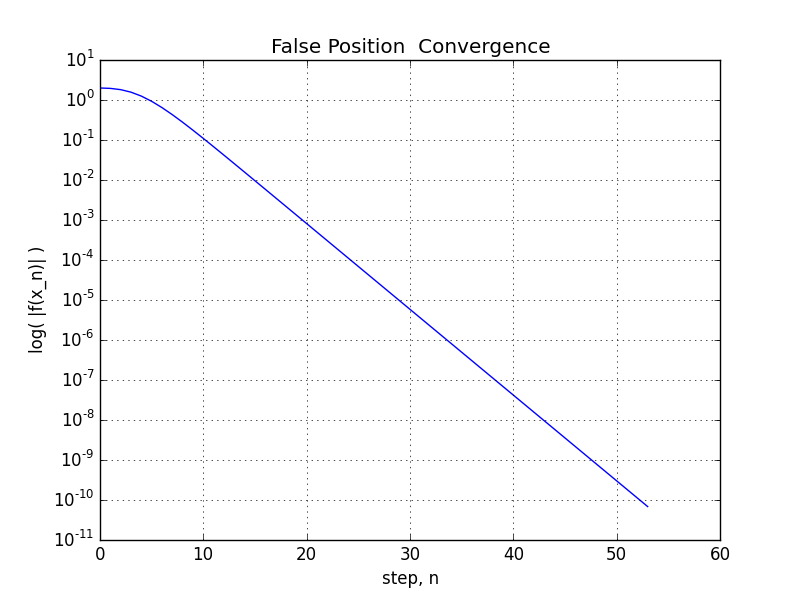
\includegraphics[width=0.75\textwidth]{Problem4c.png}
    \caption{Converges quadratically}
  \end{figure}

  \clearpage 

  \subsection{Fixed Point Iteration}
  \lstinputlisting[language=Python, firstline=2, lastline=28]{Problem4c.py}

  Using these three differnt forms for $g(x)$:\\
  \begin{align}
    \label{eq:g1}
    g_1(x) &= \frac{x}{2} + \frac{1}{x^3} \\
    \label{eq:g2}
    g_2(x) &= \frac{2x}{3} + \frac{2}{3x^3} \\
    \label{eq:g3}
    g_3(x) &= x - \frac{2}{5}(x^4-2)
  \end{align}

  \begin{figure}[h]
    \centering
    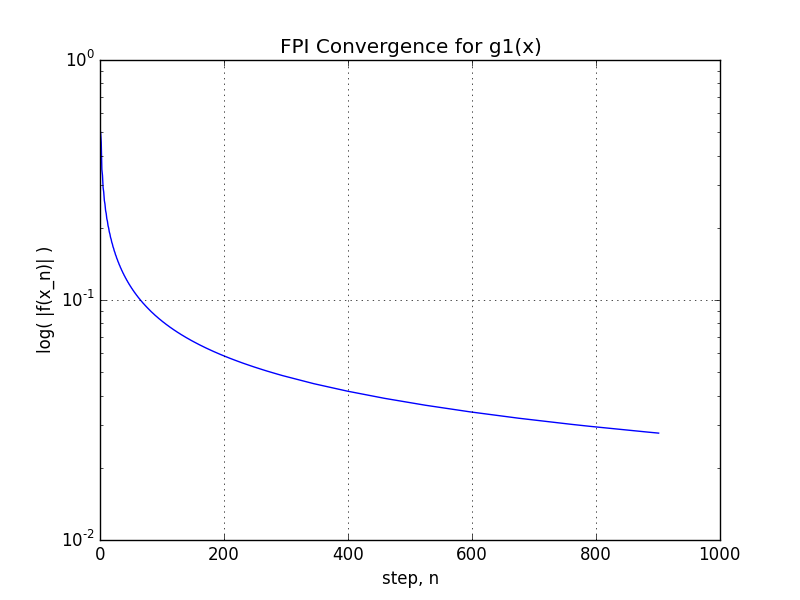
\includegraphics[width=0.7\textwidth]{Problem4da.png}
    \caption{See Eq. \ref{eq:g1}. Converges to 0.02, not very precise}
  \end{figure}


  \begin{figure}[h]
    \centering
    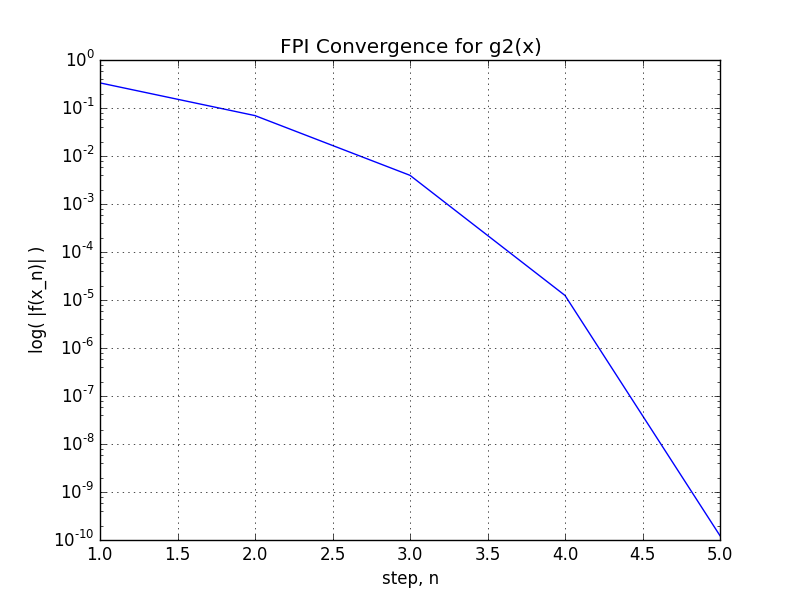
\includegraphics[width=0.7\textwidth]{Problem4db.png}
    \caption{See Eq. \ref{eq:g2}. Converges increasingly faster and only takes 5 steps to hit
            desired precision}
  \end{figure}


  \begin{figure}[h]
    \centering
    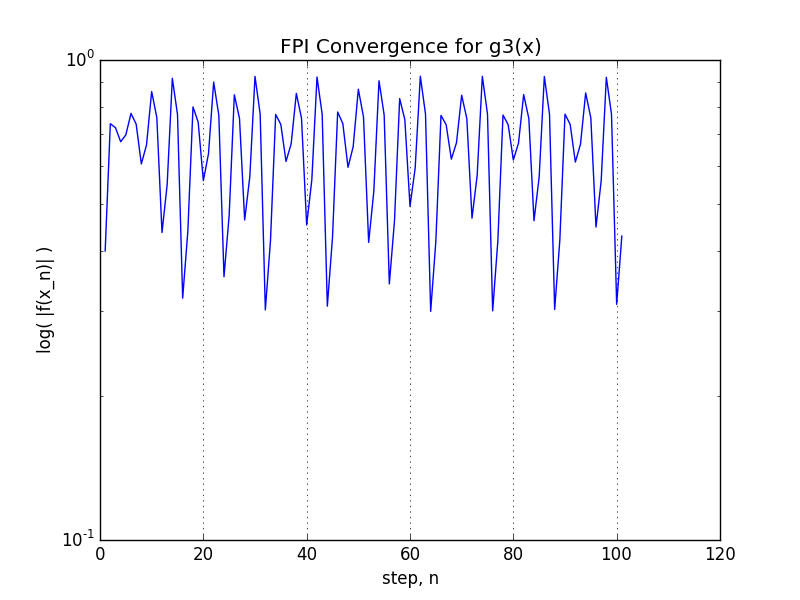
\includegraphics[width=0.7\textwidth]{Problem4dc.png}
    \caption{See Eq. \ref{eq:g3}. Oscillates around 0.5, not accurate or precise}
  \end{figure}

  \clearpage

  \section{More FPI}

  \begin{align}
    \label{eq:quad}
    f(x) &= 2x^3 - 6x -1
  \end{align}
  To find the roots of Eq. \ref{eq:quad}, we write $f(x)$ as $f(x)=x-g(x)=0$
  where possible forms of $g(x)$ are:
  \begin{align}
    \label{eq:g1}
    g_1(x) &= \frac{1}{2x^2-6} \\
    \label{eq:g2}
    g_2(x) &= \frac{3}{x}+\frac{1}{2x^2} \\
    \label{eq:g3}
    g_3(x) &= \sqrt[3]{3x + \frac{1}{2}}
  \end{align}

  Each equation gives a root of Eq. \ref{eq:quad}. All equations converge
  quadratically.\\
  $g_1(x)$ converges to $-0.16825440$\\
  $g_2(x)$ converges to $-1.64177875$\\
  $g_3(x)$ converges to $1.8100379292$

  \begin{figure}[h]
    \centering
    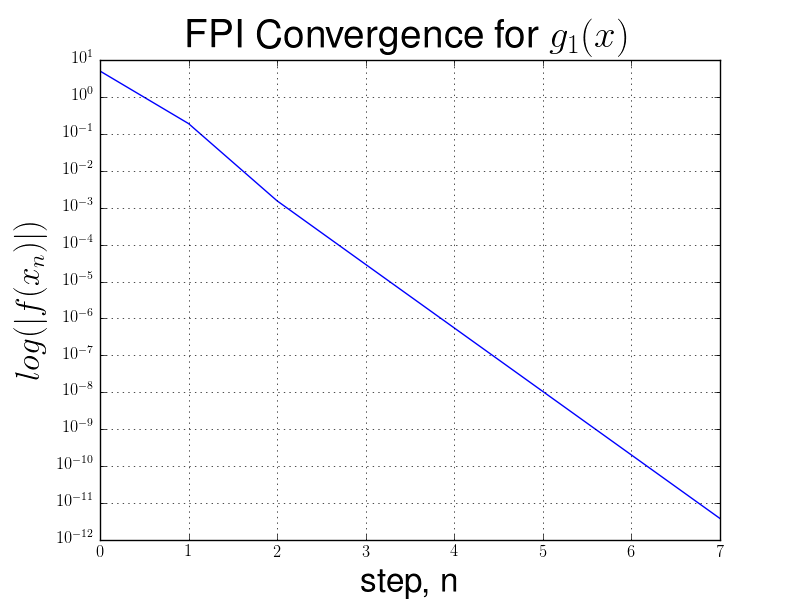
\includegraphics[width=0.7\textwidth]{Problem5a.png}
    \caption{See Eq. \ref{eq:g1}}
  \end{figure}
  
  \begin{figure}[h]
    \centering
    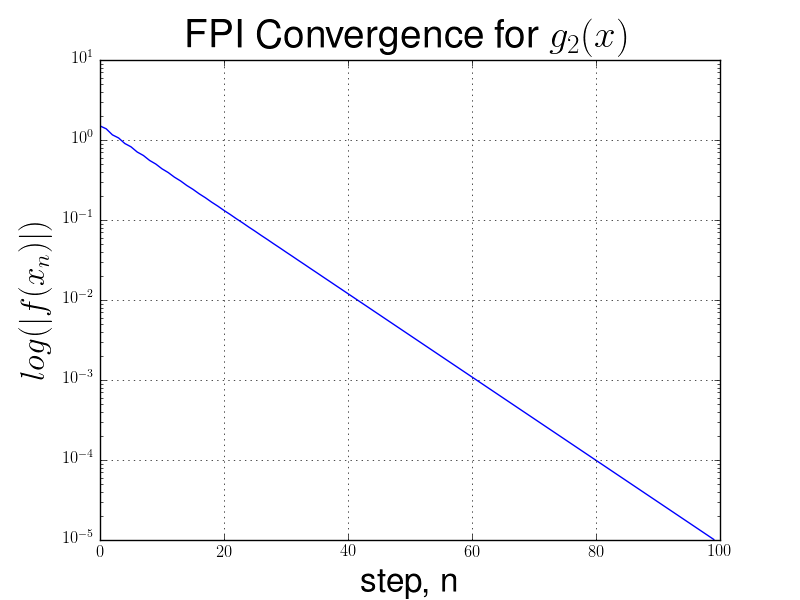
\includegraphics[width=0.7\textwidth]{Problem5b.png}
    \caption{See Eq. \ref{eq:g2}}
  \end{figure}

  \begin{figure}[h]
    \centering
    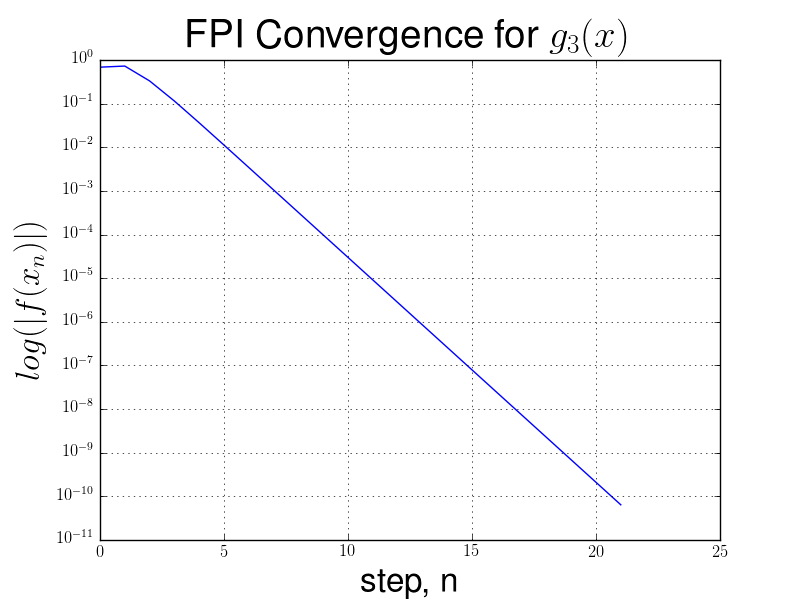
\includegraphics[width=0.7\textwidth]{Problem5c.png}
    \caption{See Eq. \ref{eq:g3}}
  \end{figure}

  \clearpage

  \section{Secants behaving badly}

  By attempting to find the root of $\Omega_1 - \Omega_2$ with the secant method,
  its possible that the brackets may try to converge on one of the two
  asymptotes.
  An better method of finding the root of this equation is to take the inverse
  and solve for its root. The inverse will asymptote on the zero of the 
  function, but the secant method will still converge on this value.
  See figure \ref{fig:omega}.

  \begin{figure}[h]
    \label{fig:omega}
    \centering
    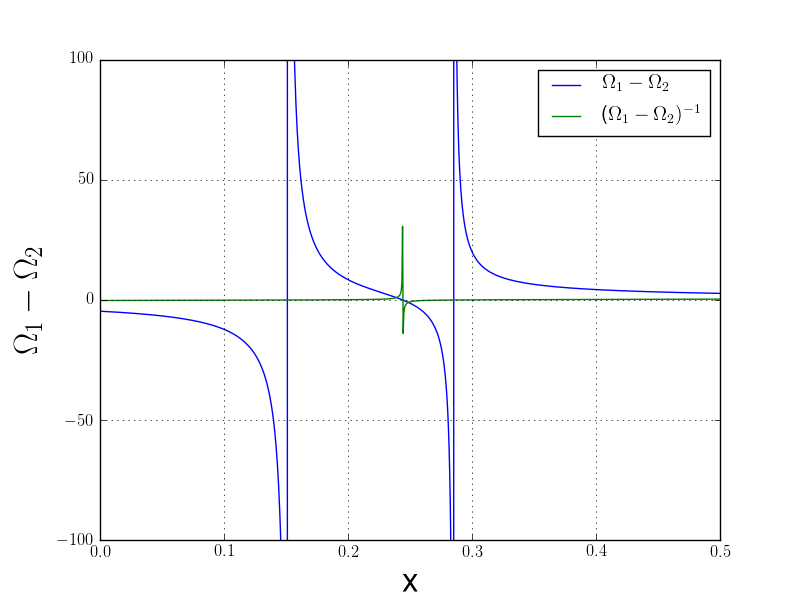
\includegraphics[width=0.7\textwidth]{Problem6a.png}
    \caption{The difference of the two functions results in three possible
    values to converge on for the secant method where their inverse gives
    only the correct one.}
  \end{figure}
  

  \clearpage
  
  \section{Convergence, or the lack thereof}

  \lstinputlisting[language=Python, lastline=14]{Problem7.py}

  
  Running until the error with the known value is less $10^{-9}$:
  \lstinputlisting{Problem7a.out}
  
  Running until the relative error between terms $n$ and $n+1$ is less than $10^{-15}$:
  \lstinputlisting{Problem7b.out}


  For $x=2$, the difference in terms quickly diminishes before a reasonable
  approximation can be made.
  \\
  For $x=-2$, the relative error never reaches the threshold where the 
  difference in terms only makes 39 steps and still produces a close
  approximation.
  \\
  For $x=-12$, both methods hit the step limit and produce the same approximation.

  \lstinputlisting{Problem7c.out}
  
  The precision for $x_0=20$ is not particularly good, though  its accuracy
  indicates that it will eventually converge to a more precise answer. For larger
  magnitudes of $x_0$, many more iterations are required until the factorial
  in the denominator reaches a large enough number that will result in small
  terms capable of converging on a precise value.
  For $x_0=-20$, this problem is even more apparant as each term will alternate
  between positive and negative. The terms can also decay in size very quickly
  resulting in an approximation that decays more and more slowly away from a
  very innacurate estimate, as is in the case of $x_0=-20$.

  

  \clearpage

  \section{Multidimensional Newton's Method}

  \begin{align}
    \label{eq:Q}
    V(B+W)^2 - S\frac{B+2W}{W^2}=Q \\
    \label{eq:N}
    -\frac{B}{2}(1+V)+\frac{S}{2}W^{-2}-W+\frac{1}{2}\left[(1-V)W-D\sqrt{1-V}\right]=N
  \end{align}

  Solve  Eq. \ref{eq:Q} for $V(W)$:

  \begin{align}
    \label{eq:V(W)}
    V = \frac{Q}{(B+W)^2} + S\frac{B+2W}{W^2(B+W)^2}
  \end{align}

  And substitute Eq. \ref{eq:V(W)} into Eq. \ref{eq:N} and set it to 0:
  
  \begin{align}
    -\frac{B}{2}(1+\frac{Q}{(B+W)^2} + S\frac{B+2W}{W^2(B+W)^2})+\frac{S}{2}W^{-2}-W\nonumber\\
+\frac{1}{2}\left[(1-V)W - D\sqrt{1-\frac{Q}{(B+W)^2} + S\frac{B+2W}{W^2(B+W)^2}}\right]-N=0
  \end{align}

  \clearpage

  \section{Blackbody Radiation}
  
  \begin{align} 
    e^{h\nu / k_B T} &= 1 + \frac{h \nu}{k_B T} + \cdots \nonumber \\
    u(\nu, T) &= \frac{dU}{d\nu} =
    \frac{8\pi h \nu^3}{c^3}\frac{1}{e^{h\nu/k_B T}-1} \nonumber \\
    u(\nu, T) &= \frac{dU}{d\nu}  =
      \frac{8\pi h \nu^3}{c^3}\frac{k_B T}{h \nu} \nonumber \\
    \label{eq:nu}
    u(\nu, T) &= \frac{dU}{d\nu}  =
      \frac{8\pi \nu^2 k_B T}{c^3 }
  \end{align}

  \begin{figure}[h]
    \centering
    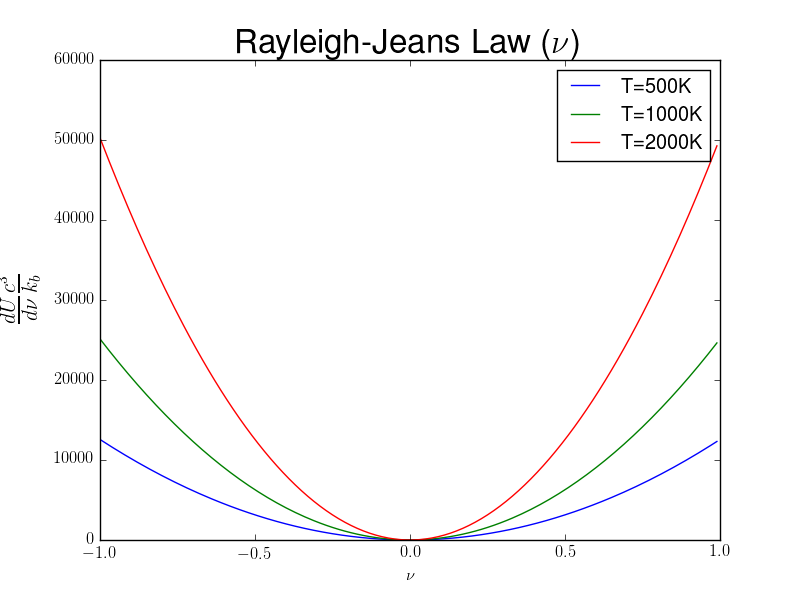
\includegraphics[width=0.8\textwidth]{Problem9a.png}
    \caption{See Eq \ref{eq:nu}}
  \end{figure}

  \clearpage

  Or in terms of $\lambda$, where $\lambda \equiv \frac{c}{\nu}$

  \begin{align}
    \frac{dU}{d\nu}\frac{d\nu}{d\lambda} &= \frac{d\nu}{d\lambda}\left[\frac{8\pi h \nu^3}{c^3 }\frac{1}{e^{h\nu/k_BT}-1}\right] \nonumber\\
    \frac{d\nu}{d\lambda} &= \frac{d}{d\lambda}\left(\frac{c}{\lambda}\right) = -\frac{c}{\lambda^2} \nonumber\\
    \frac{dU}{d\lambda} &= \left(-\frac{c}{\lambda^2}\right)\left[\frac{8\pi h}{\lambda^3}\frac{1}{e^{hc/k_BT\lambda}-1}\right] \nonumber\\
    \frac{dU}{d\lambda} &= \left(-\frac{c}{\lambda^2}\right)\left[\frac{8\pi h}{\lambda^3}\frac{k_BT\lambda}{hc}\right] \nonumber\\
    \label{eq:lambda}
    \frac{dU}{d\lambda} &= \frac{8\pi k_BT}{\lambda^4}
  \end{align}

  
  \begin{figure}[h]
    \centering
    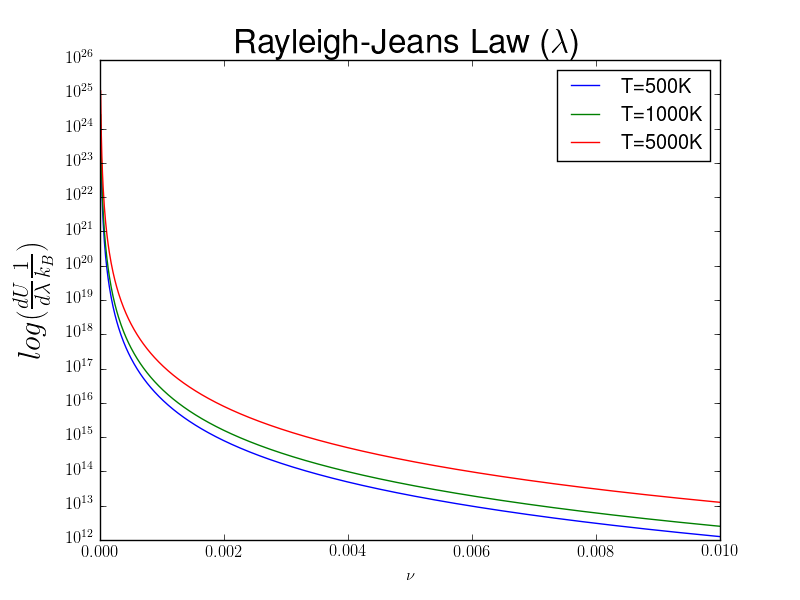
\includegraphics[width=0.8\textwidth]{Problem9b.png}
    \caption{See Eq \ref{eq:lambda}}
  \end{figure}

  \clearpage

  \begin{align}
    u(x,\hat{T}) = \frac{8\pi h \nu_0^3}{c^3}\hat{T}^3\frac{x^3}{e^x-1} \nonumber
  \end{align}
  Where $\hat{T} \equiv \frac{T}{T_0}$, $\hat{\nu} \equiv \frac{\nu}{\nu_0}$,
  $\hat{\lambda} \equiv \frac{\lambda}{\lambda_0}$ and $x \equiv \frac{\hat{\nu}}{\hat{T}} = \frac{h\nu}{k_BT}$

  \begin{align}
    \frac{du(x,\hat{T})}{dx} = -\frac{8\pi h \nu_0^3}{c^3}\hat{T}^3\frac{(e^x(x-3)+3)x^2}{(e^x-1)^2} \nonumber
  \end{align}

  
\end{document}
